\documentclass[12pt, twosided]{report}  % type of Documents


%_____________________________________PACKAGES__________________________________
\usepackage[utf8]{inputenc} % input encoding [utf8]
\usepackage[english]{babel} % setting spell-check for English
\usepackage{geometry} % for page margins
\usepackage{fancyhdr} % for header and footer
\usepackage{url} % package to include urls
\usepackage{datetime} % For inserting date and time
\usepackage{graphicx} % For inserting graphics
\usepackage{float} % for accurate placement of figures and tables
\usepackage[labelfont=bf,textfont=bf]{caption} % for having the captions in bold
\usepackage{amsmath} %for equations
\usepackage[hidelinks]{hyperref} % for adding hyperlinks (withouht ugly boxes)
\usepackage{nomencl} % For Nomenclature 
\makenomenclature
\usepackage{amssymb} % symbols for nomenclature
\usepackage{etoolbox} % For Creating Categories in Nomenclature
\usepackage{caption} % For subfigures
\usepackage{subcaption} % For subfigures

%_______________________________________________________________________________


% PAGE GEOMETRY
\geometry{left=1cm,right=1cm,top=1cm,bottom=1cm,includeheadfoot}


%_____________________________HEADER AND FOOTER_______________________
\fancypagestyle{mypagestyle}{
\fancyhead{}
\fancyfoot{}
\fancyhead[L]{\rightmark}
\fancyhead[R]{SARS-CoV-2: A Summary of Situation}
\fancyfoot[R]{\today}
\fancyfoot[C]{\thepage}
\fancyfoot[L]{Divyansh Chahar}
\renewcommand{\headrulewidth}{0pt}
\renewcommand{\footrulewidth}{0.8pt}
}
%_____________________________________________________________________


%____________________________________________NOMENCLATURE____________________________
\renewcommand\nomgroup[1]{%
	\ifstrequal{#1}{A}{\item[\Large\bfseries{Greek Characters}]}{%
	\ifstrequal{#1}{B}{\vspace{10pt} \item[\Large\bfseries{Roman Characters}]}{%
	\ifstrequal{#1}{C}{\vspace{10pt} \item[\Large\bfseries{Acronyms}]}{}}}%
}
%____________________________________________________________________________________

\pagestyle{mypagestyle} % For Header and Footer
\renewcommand\thesection{\arabic{section}} % Section Numbers Stating From 1
\renewcommand{\thefigure}{\thesection-\arabic{figure}} % to include section numbers in figures

%%%%%%%%%%%%%%%%%%
%%% TITLE PAGE %%%
%%%%%%%%%%%%%%%%%%

\begin{document}
	\begin{titlepage}
		\newgeometry{a4paper,top=3cm,bottom=1cm,right=3cm,left=3cm} % Setting Page Dimensions
		\begin{center}
			{\LARGE \textbf{SARS-CoV-2}}\\
			
			\hrulefill
		
			\textbf{A Summary of Situation}
			
			\null
			
			Divyansh Chahar
			
			\vfill
			
			\href{https://www.linkedin.com/in/divyanshchahar/}{
\includegraphics[width=0.25\linewidth]{./images/icons/my_qrcode.eps}}
		
			\null
		
			\href{https://www.linkedin.com/in/divyanshchahar/}{
\includegraphics[width=0.025\linewidth]{./images/icons/linkedin_logo.eps}}
			\href{https://www.linkedin.com/in/divyanshchahar/}{https://www.linkedin.com/in/divyanshchahar/}
			
			\null
			
			\href{https://www.linkedin.com/in/divyanshchahar/}{
\includegraphics[width=0.025\linewidth]{./images/icons/github_mark.eps}}
			\href{https://github.com/divyanshchahar}{https://github.com/divyanshchahar}
			
			\vfill
			
			\today
			
		\end{center}
	\end{titlepage}


\restoregeometry

%%%%%%%%%%%%%%%%%%%%%%%
%%%	NOMENCLATURE	%%%
%%%%%%%%%%%%%%%%%%%%%%%
\printnomenclature

\pagebreak

%%%%%%%%%%%%%%%%%%%%%%%
%%% MAIN CONTENT	%%%
%%%%%%%%%%%%%%%%%%%%%%%

\section{Introduction}
The previous report analyzed the spread of infection, this report will focus on analyzing the situation in the ten countries with highest number of Coronavirus cases. These countries have different demographics, are located in different continents, and have different levels of healthcare infrastructure. Different factors affect the impact of Coronavirus in different countries. The first Major outbreak outside of China was recorded in Italy, Italy has the seventh highest number of Coronavirus cases but has recorded the fourth highest number of deaths. This disproportionate amount of deaths could be due to the age distribution of Italy's population, such parameters can't be measured through the database which is used in this report, however the effect of such factors could be measured through various parameters like mortality factor, recovery ratio etc.
\\
\\
This report will focus on the some new parameters which are described in the next section.

\section{Parameters Under Consideration}
\subsection*{Number of Deaths and Recovered Cases}
The number of deaths and recovered cases will always be proportional to the number of confirmed cases. A comparative Analysis of these numbers can highlight disproportionalities which would otherwise be hidden.
\subsection*{Mortality Factor}
Mortality Factor is the ratio of deaths to cases of infection. A country which has higher number of cases might also have higher number of deaths. Therefore a comparison of ratios between data sets of different population size can represent a better picture. It can be mathematically represented as
$$\beta=\frac{\sum^{i=0}_{t} I_n}{\sum^{i=0}_{t} D_n}$$
\nomenclature[B]{$\beta$}{mortality facotr}
\nomenclature[A]{$I$}{number of infected individuals}
\nomenclature[A]{$D$}{number of deaths}
\nomenclature[A]{$t$}{time} 
\subsection*{Recovery Ratio}
Similar to Mortality Factor, Recovery Ratio also helps in better understanding of number of recovered individual in data sets of different population sizes. This is more important than mortality factor. The countries which will become the foci of this report in a later section, majority of them reported higher number of recovered cases than deaths. Recovery Ratio can be expressed as
$$\sigma=\frac{\sum^{i=0}_{t} I_n}{\sum^{i=0}_{t} R_n}$$
\nomenclature[B]{$\sigma$}{recovery ratio}
\nomenclature[A]{$R$}{Number of Recovered Cases}
\\
As mentioned in \cite{kermack1927contribution} reproduction number is inversely proportional to the cases which can no longer be infected. Although the number of deaths is a factor which  contributes to this, but the majority of contribution comes from the cases which have recovered. Thus recovery ratio is not only a measure of how good a country's response is to the situation.
\subsection*{Log-Log Curve}
Log-Log Curve is a method and not a numerical parameter that can be calculated. In this method, number of new cases are plotted against number of confirmed cases, but both x and y axis use a logarithmic scale. This method is particularly helpful due to the numerical nature of spread of infectious disease. As mentioned in \cite{chowell2016growing}, spread of infectious disease follows an exponential growth phase in the beginning. This growth pattern can be simulated using the the equation from \cite{Abramson2015}
$$y=ae^{kt}$$

\nomenclature[A]{y}{value at time $t$}
\nomenclature[A]{$A_0$}{value at time $t=0$}
\nomenclature[A]{k}{growt/decay Rate}
\nomenclature[A]{t}{time interval in days}

\begin{figure}[H]
\centering

	\begin{subfigure}[b]{0.5\textwidth}
		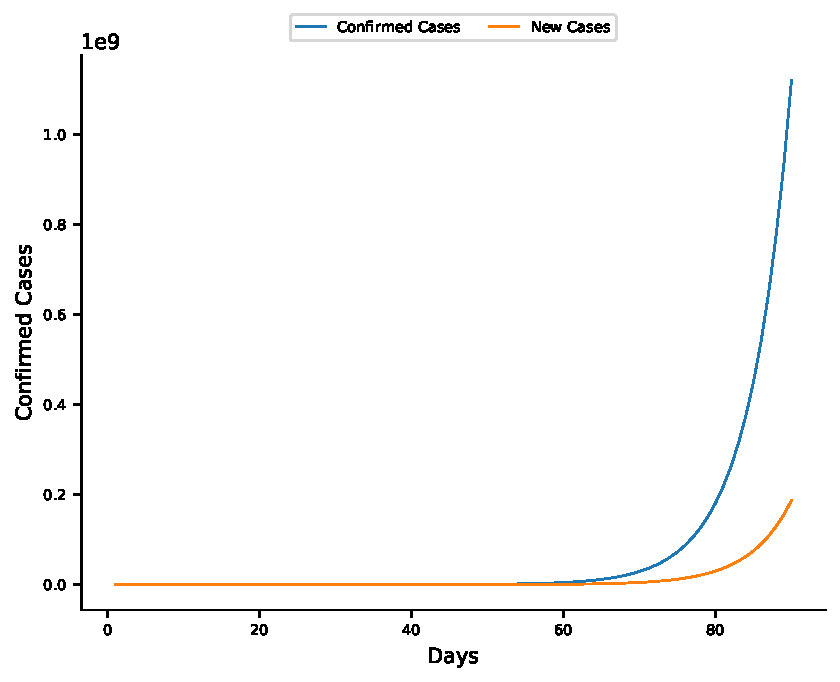
\includegraphics[width=\textwidth]{./images/plot_11.pdf}
		\subcaption{sustained Growth Rate}
		\label{plot_sustained}
	\end{subfigure}

	\begin{subfigure}[b]{0.25\textwidth}
		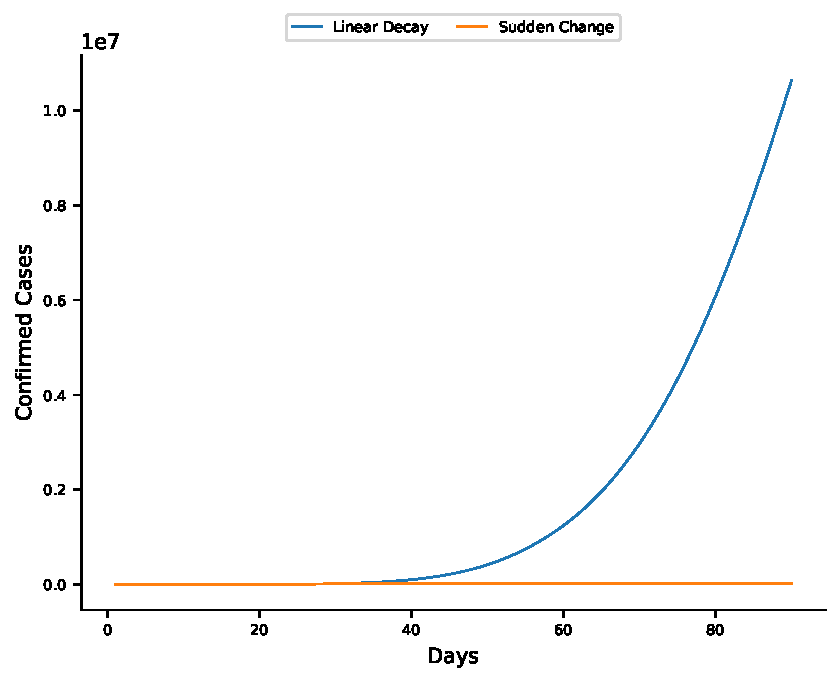
\includegraphics[width=\textwidth]{./images/plot_12.pdf}
		\subcaption{Changing Growth Rate}
		\label{plot_changinggrowthrate}
	\end{subfigure}
	\begin{subfigure}[b]{0.25\textwidth}
		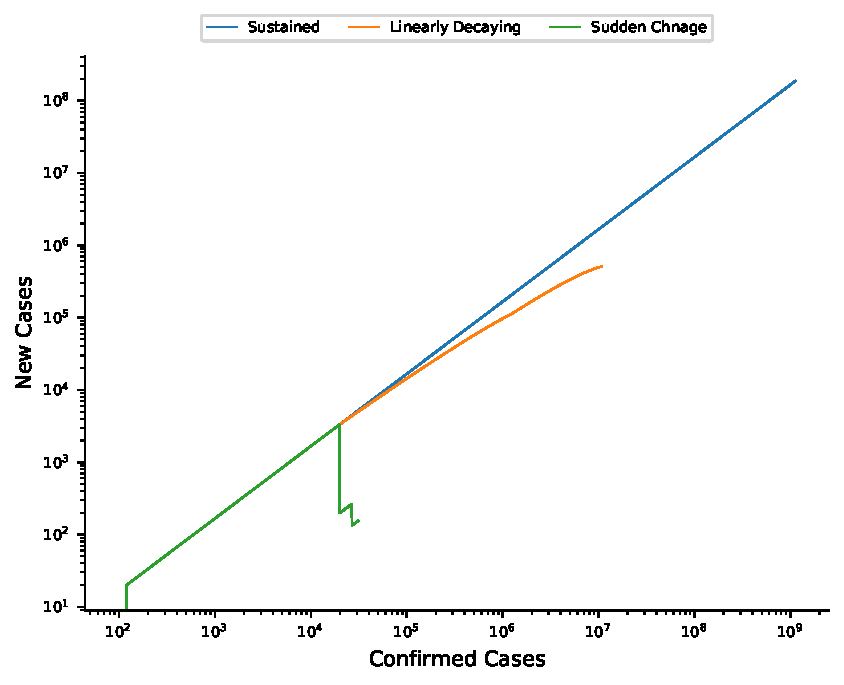
\includegraphics[width=\textwidth]{./images/plot_13.pdf}
		\subcaption{Behaviour on log-log curve}
		\label{plot_behavioursimulated}
	\end{subfigure}
\caption{Simulated spread of epidemic}
\label{plot_simulated}
\end{figure}


Using the Above equation, three scenarios were simulated follows:
\begin{itemize}
	\item \textbf{Sustained Growth Rate:} In this scenario the number of cases increase by 20\% at the end of each time cycle. This Growth Rate is maintained for the entire 90 days. This scenario mimics an uncontrollable spread of infectious disease. It represents a situation when an infectious disease spreads rapidly and no countermeasures are either introduced or fail to be effective
	\item \textbf{Linearly Decaying Growth Rate:} This scenario follows a 20\% Growth Rate for first 30 days, at $31^{st}$ day the growth rate starts decreases linearly to 10\% over the next 30 days, and then to 2.5\% over the another 30 days.This scenario mimics an uncontrollable spread of an infectious disease for 30 days without any counter measures, then first set of counter measures are introduced, and the growth rate falls to 10\% over the next 30 days, on $61^{st}$ day more strict counter measures are deployed and the growth rate eventually falls to just 2.5
	\% over the next 30 days.   
	\item \textbf{Sudden Change in Growth Rate:} For the simulation, uncontrolled outbreak was simulated for first 30 days with a 20\% growth rate. On $31^{st}$ day strict measures are taken to control the spread of virus resulting in the growth rate being reduced 1\% for the next 30 days, on $61^{st}$ day, another round of strict measures are imposed and the growth rate falls to  0.5\%. 
\end{itemize}

It must be noted that the three scenarios simulated above are exaggerated text-book examples, although the spread of infection follows a growth pattern similar to the above mentioned examples, but the plots for real data will not exactly be like any of the plots in figure \ref{plot_simulated}
\\
\\
It can be observed from figure \ref{plot_sustained}, that new cases as well as confirmed cases both increase exponentially as time progresses, thus it is justifiable to use logarithmic axis when plotting both these numbers against each other.
\\
\\
Figure \ref{plot_changinggrowthrate} illustrates the vast difference between gradual and sudden change in growth rate. When comparing figure \ref{plot_sustained} and figure \ref{plot_changinggrowthrate}, it can be observed that for sustained growth rate the slope increases very rapidly and becomes near vertical where as in case of linearly decaying growth rate the increase in slope is not as aggressive. It must be noted for sudden change in growth rate the line remains almost flat, this highlights how effective strict measures can be if implemented early during the spread of infection and if followed sincerely.
\\
\\
An interesting pattern can be observed in figure \ref{plot_behavioursimulated}, for sustained growth rate, the curve is a straight line, indicating that both the number of new cases and confirmed cases are increasing in a similar manner, for linearly decaying growth rate, the curve starts to flatten, indicating that new cases are not rising as quickly as new cases. For sudden change in growth rate, a steep drop can be observed, this highlight huge difference between the growth pattern of new and confirmed cases, due to sudden drop in growth rate the amount of new cases drop significantly as the count of confirmed cases continue to rise. Further in this report this pattern will be observed for some countries. It is the most important indicator which highlights weather the exponential growth has stopped or not.
\pagebreak
\section{Comparitive Analysis}
The database used in this report is maintained by John Hopkins University, the version used in this report was last updated on $10^{th}$-June-2020.
\begin{figure}[H]
	\centering
	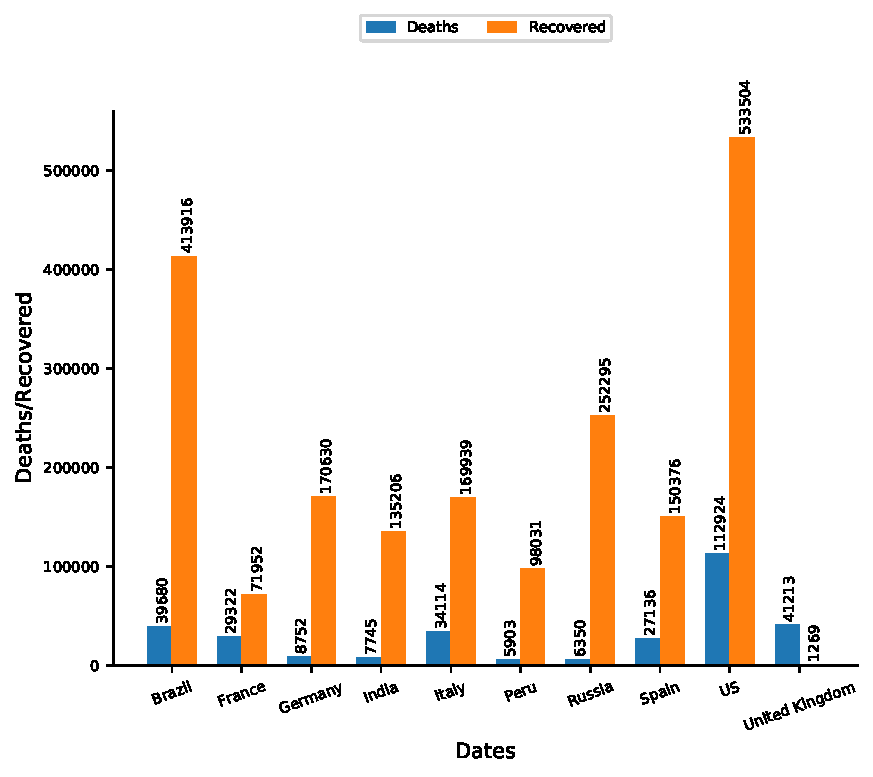
\includegraphics[width=0.5\textwidth]{./images/plot_1.pdf}
	\caption{Number of Deaths and Recovered Cases}
	\label{plot_deathrecovered}
\end{figure}

As can be observed from figure \ref{plot_deathrecovered}, USA has the highest number of deaths and recovered cases. United Kingdom ranks fourth in term of number of cases but has the second highest number of deaths, also it is the only country where number of deaths is higher than the number of people who have recovered. Italy has the seventh highest number of coronavirus cases, but the death toll is fourth highest. France and Geramny have fifth and seventh highest amount of deaths but have ninth and tenth highest amount of confirmed cases respectively. The countries mentioned above rank higher in terms of number of deaths but rank lower in terms of confirmed cases.
\\
\\
The countries which rank higher in terms of confirmed cases but rank relatively lower in terms of  deaths are Brazil, Russia, India and Peru. The most significant difference can be seen in case of Russia, which has the third highest highest number of cases but ninth highest number of deaths. India has the fifth highest amount of cases but has eighth highest number of deaths. Similar observation can be made for Peru, which is eighth in number of cases but ranks tenth in number of deaths
\\
\\
A similar pattern can be observed for the number of recovered cases as well. India and United Kingdom have the fifth and fourth highest number of confirmed cases but ranks seventh and tenth in terms of recovered cases.
\\
\\
Germany and Italy have the tenth and seventh highest number of cases but rank fourth and fifth in term of recovered cases respectively.

\begin{figure}[H]
	\centering
	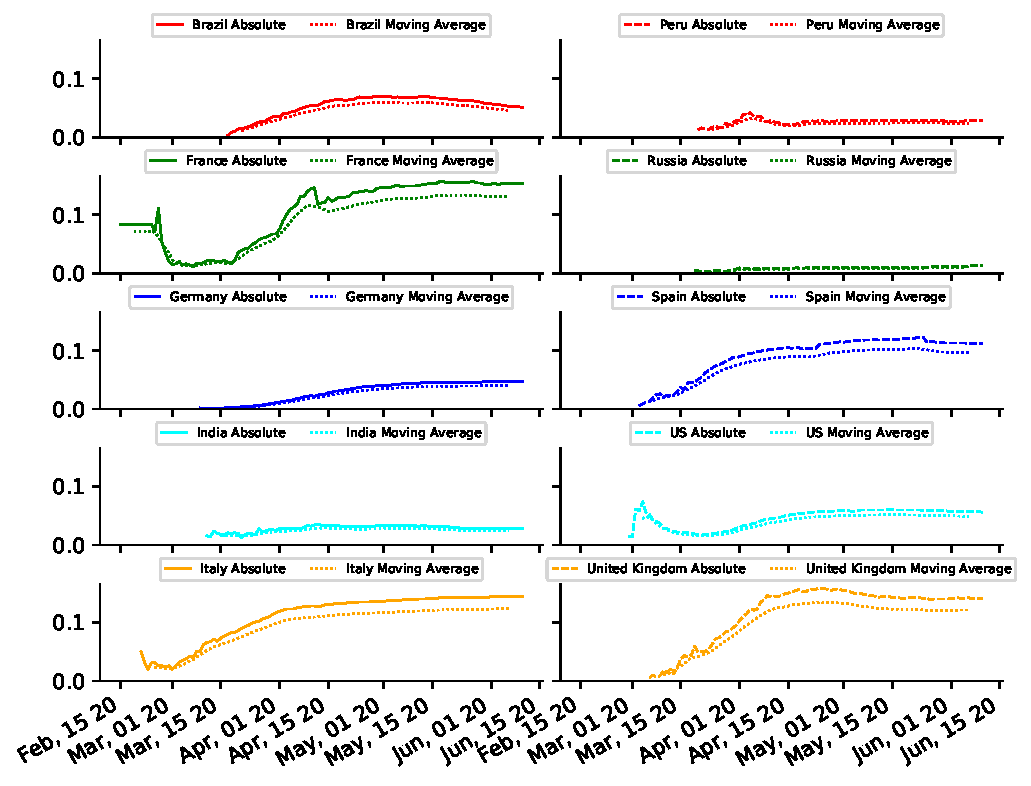
\includegraphics[width=0.5\textwidth]{./images/plot_7.pdf}
	\caption{Mortality Factor trends of 10 countries worst affected by Coronavirus}
	\label{plot_mortalityfactor}
\end{figure}

Although figure \ref{plot_deathrecovered}, gives a perspective of the number of deaths and recovered cases, but this report compares countries with significant amount of difference in the number of confirmed cases, thus there is a need to compare ratios rather than numbers. Hence Mortality Factor is used to normalize the number of deaths in a country.
\\
\\
US has the highest number of deaths but the mortality factor in US is fifth highest, which is still lower than Spain, United Kingdom, Italy and France. Similarly United Kingdom has the second highest number of deaths but mortality factor is third highest. Brazil has the third highest number of deaths but mortality factor is fifth highest. Italy and France have the fourth and fifth highest number of deaths, but mortality factor is the first and second highest respectively. Among the worst hit countries Russia has the minimum mortality factor. See figure \ref{plot_1} for progression of Mortality Factor.
\\
\\
It can be observed from figure \ref{plot_mortalityfactor}, that mortality factor rises as time progress. For majority of countries the curve for mortality factor flattens out as time progress, even though mortality factor is comparatively low in the beginning, it climbs quickly. India, US and Peru are an exception to this trend in mortality factor. India and Peru did not observe high mortality factor as compared to other countries, also no steep slope is observed for these countries. US also observes low mortality factor as compared to other countries, but lowest mortality factor is observed around march 15, then the curve rises to higher values and flattens out. Germany and Brazil also do not observe a steep slope in mortality factor, but mortality factor is much higher in Brazil than in Germany. Steepest slope and highest numbers for mortality factor are observed for United Kingdom, France, and Italy.

\begin{figure}[H]
	\centering
	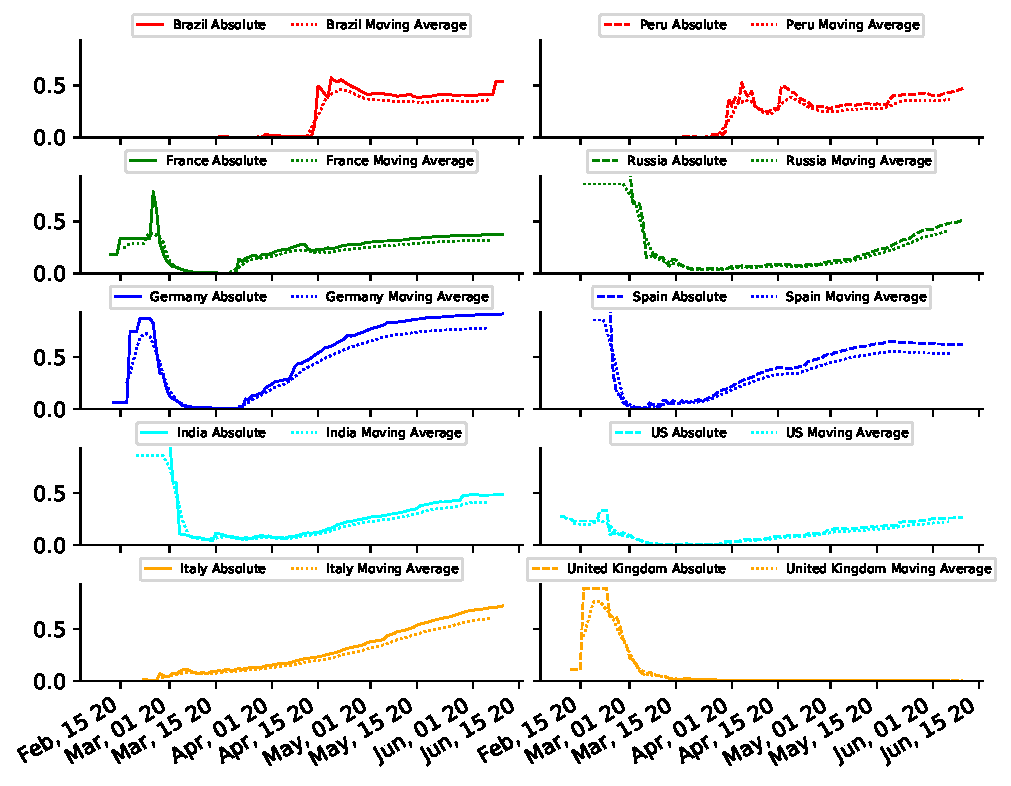
\includegraphics[width=0.5\textwidth]{./images/plot_5.pdf}
	\caption{Recovery Ratio trends of 10 countries worst affected by Coronavirus}
	\label{plot_recoveryratio}
\end{figure} 

Figure \ref{plot_recoveryratio} shows recovery ratio for the countries under analysis. A plot for better comparative analysis is shown in figure \ref{plot_2}. From figure \ref{plot_2} we can see that US has the second lowest recovery ratio despite having the highest numbers in recovered cases. Brazil on the other hand has the second highest number of recovered cases but when normalized by number of cases Brazil ranks fourth in recovery ratio. Similarly Russia Ranks third in terms of number but when normalized it ranks fifth. Germany and Italy have the fourth and fifth highest number of recovered cases, but hold the top two spots for recovery ratio. The recovery ratio is lowest for United Kingdom.
\\
\\
Change in recovery ratio over time can be observed from figure \ref{plot_recoveryratio}. Italy is the only country where recovery ratio shows a clear upward trend over the time period. Germany which developed the highest recovery ratio over time, observes a time period where recovery ratio falls to almost zero. This pattern can be observed for Germany, US and France. Among these three countries US has the shortest time period where recovery ratio falls to almost zero. A period of low recovery ratio can be observed can be observed for Russia and India, but in these two countries recovery ratio does not falls or comes as close to zero as compared to France, US and Germany. United Kingdom has the lowest recovery ratio amongst all the countries under consideration. It can be observed that for United Kingdom recovery ratio falls to extremely low levels as time progresses. Extremely low recovery ratio and high mortality factor, has resulted in United Kingdom having higher deaths than recovered cases.

\begin{figure}[H]
	\centering
	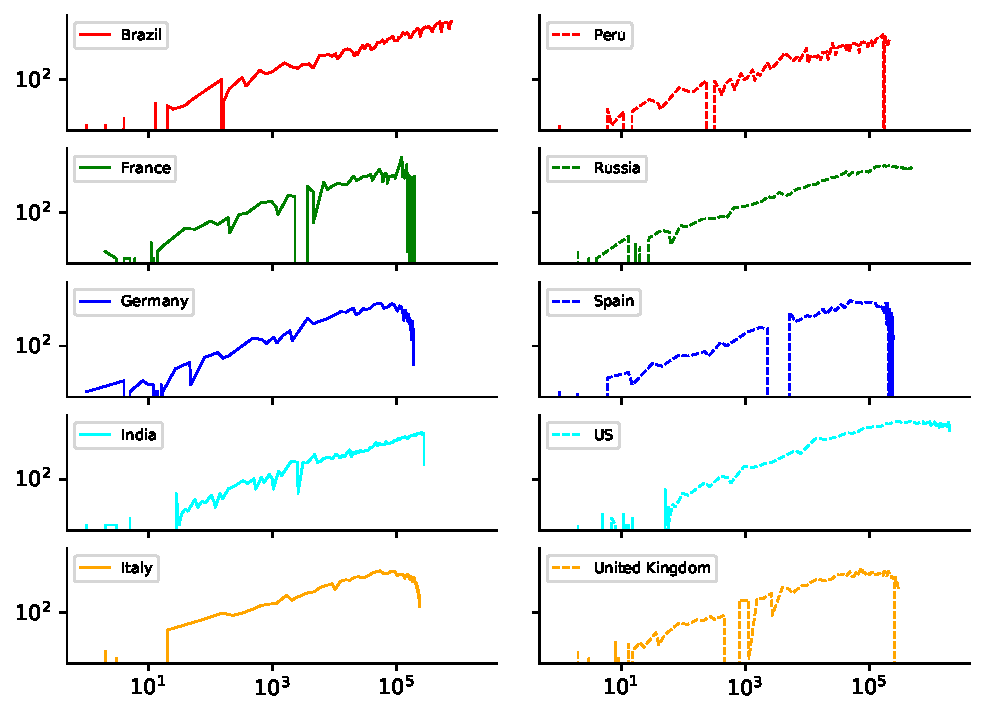
\includegraphics[width=0.5\textwidth]{./images/plot_9.pdf}
	\caption{Log-Log curve for 10 countries worst affected by Coronavirus}
	\label{plot_loglogactual}
\end{figure} 

As mentioned in the previous section Log-Log Curve can give a better over all picture of the the situation. From figure \ref{plot_loglogactual}, it can be observed that Germany, India and Italy exhibit a clear trend which is similar to sudden change in growth as shown in figure \ref{plot_behavioursimulated}. Germany and Italy exhibit oscillatory behavior towards the end of the curve, but exhibit an over all downward trend. However this pattern in not seen for India, which exhibit a clear sudden fall in the curve. Sudden downfall towards the end of the curve can also be observed for United Kingdom, Spain, Peru and France, but it can't be conclusively classified as sudden change in growth rate. For United Kingdom and Peru, sharp decline in the curve can be observed towards the end of the curve, but on closer observation it can be seen that the curve returns to the previous slope immediately. A sharp decline towards the end of the curve can also be observed for France and Spain, but it can't be conclusively said that spread of virus is not following an exponential growth pattern in these two countries because, huge oscillations towards the end of the curve can be observed and there is no clear downward trend.

\section{Conclusion}
Based on the above observation the following conclusions can be drawn
\begin{itemize}
	\item Countries which rank higher in terms of number of confirmed cases but rank lower in number of deaths have a lower mortality factor compared to the countries which rank lower in terms of number of confirmed cases but rank higher in terms of number of deaths. The only exception to this rule is Brazil.
	\item Countries which rank higher in terms of number of confirmed cases but rank lower in number of recovered cases have a lower mortality factor compared to the countries which rank lower in terms of number of confirmed cases but rank higher in terms of number of recovered cases.
	\item Mortality Factor and recovery ratio are better indicators than number of deaths and recovered cases
	\item For assessing the overall situation (i.e. the nature of spread of the virus), Log-Log curve is a better indicator than growth used in \cite{divyansh_covid_1}
\end{itemize}
 

%%%%%%%%%%%%%%%%%%%%%%%
%%%	BIBLIOGRAPHY	%%%
%%%%%%%%%%%%%%%%%%%%%%%

\bibliographystyle{ieeetr}
\bibliography{myrefrences}

%%%%%%%%%%%%%%%%%%%
%%%	APPENDIX	%%%
%%%%%%%%%%%%%%%%%%%

\renewcommand{\thesection}{\Alph{section}}
\renewcommand{\thefigure}{\thesection-\arabic{figure}}
\setcounter{figure}{0}

\pagebreak
\appendix

\section{Appendix-A}

\begin{figure}[H]
	\centering
	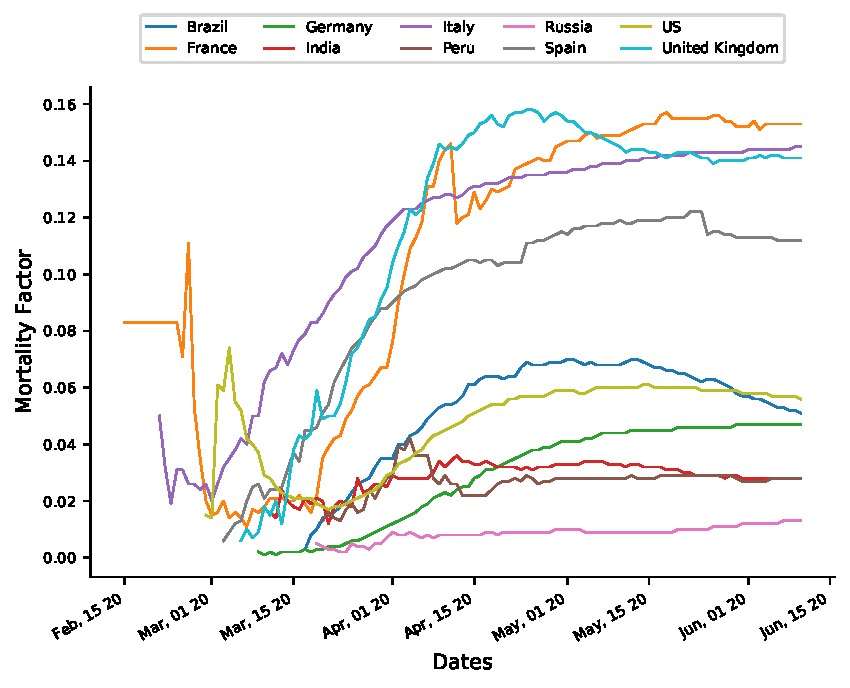
\includegraphics[width=0.5\textwidth]{./images/plot_8.pdf}
	\caption{Mortality Factor}
	\label{plot_1}
\end{figure}

\begin{figure}[H]
	\centering
	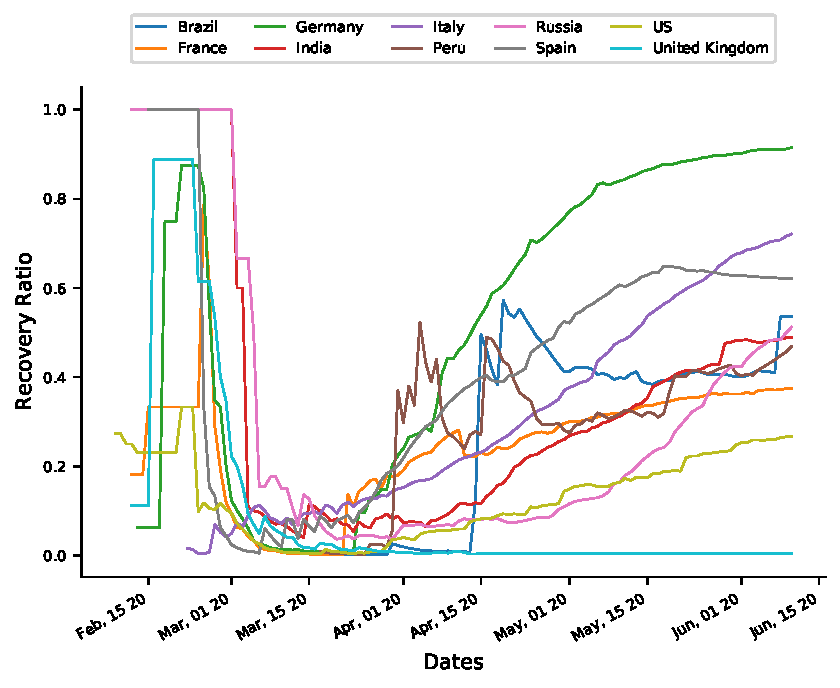
\includegraphics[width=0.5\textwidth]{./images/plot_6.pdf}
	\caption{Recovery Ratio}
	\label{plot_2}
\end{figure}

\end{document}